% ============================================================
%  sec-2-architecture-strategy.tex  —  4.2 Architecture and
%  Migration Strategy
% ============================================================

\section{Architecture and Migration Strategy}
\label{sec:architecture-strategy}

\subsection{Full Stack Migration Overview}
\label{subsec:stack-overview}

The migration replaces every \acrshort{cuda}-dependent component in
the Nemotron 3 Nano pipeline with a CANN-compatible equivalent,
while preserving the components that are hardware-agnostic. \tabref{full-stack-mapping}
documents the complete mapping.

\newcolumntype{K}{>{\raggedright\arraybackslash\ttfamily\scriptsize}X} % Use scriptsize for very long code names in tables

\begin{table}[htbp]
  \centering
  \caption{Complete CUDA-to-CANN stack mapping}
  \label{tab:full-stack-mapping}
  \begin{tabularx}{\textwidth}{l K K l}
    \toprule
    \tableheader{Layer & CUDA (Original) & CANN (Target) & Change} \\
    \midrule
    Hardware
      & NVIDIA H100 SXM5
      & Huawei Ascend 910C
      & Infrastructure \\
    \rowcolor{TableRowOdd}
    Compute runtime
      & CUDA + cuDNN + cuBLAS
      & CANN AscendCL + CANN NN Library
      & Abstracted via \texttt{torch\_npu} \\
    Distributed comm.
      & NCCL
      & HCCL
      & Backend string change \\
    \rowcolor{TableRowOdd}
    Training framework
      & Megatron-Bridge + \texttt{torchrun}
      & Megatron-Bridge + \texttt{torch\_npu} + \texttt{torchrun}
      & Patched entry point \\
    Mamba SSM kernel
      & \texttt{selective\_scan\_cuda}
      & \texttt{ops/mamba\_ascend.py}
      & New file \\
    \rowcolor{TableRowOdd}
    MoE dispatch kernel
      & Fused CUDA gather/scatter
      & \texttt{ops/moe\_routing\_ascend.py}
      & New file \\
    Mixed precision
      & \texttt{torch.cuda.amp.autocast}
      & \texttt{torch.npu.amp.autocast}
      & 10-line patch \\
    \rowcolor{TableRowOdd}
    Data preparation
      & Ray CPU (no GPU)
      & Ray CPU (unchanged)
      & None \\
    Inference engine
      & TensorRT-LLM / vLLM
      & MindIE / vLLM-Ascend
      & New compilation step \\
    \rowcolor{TableRowOdd}
    Inference server
      & Triton / NIM
      & \texttt{inference/serve.py}
      & New file \\
    Observability
      & Weights \& Biases
      & Weights \& Biases (unchanged)
      & None \\
    \rowcolor{TableRowOdd}
    Orchestration
      & NeMo-Run + Slurm
      & NeMo-Run + Slurm + \texttt{env.toml} Ascend profile
      & Config addition \\
    Containerisation
      & NVIDIA NeMo images
      & \texttt{docker/Dockerfile.sft} + \texttt{.inference}
      & New Dockerfiles \\
    \bottomrule
  \end{tabularx}
\end{table}

% Figure 4.1 placeholder
\begin{figure}[H]
    \centering
    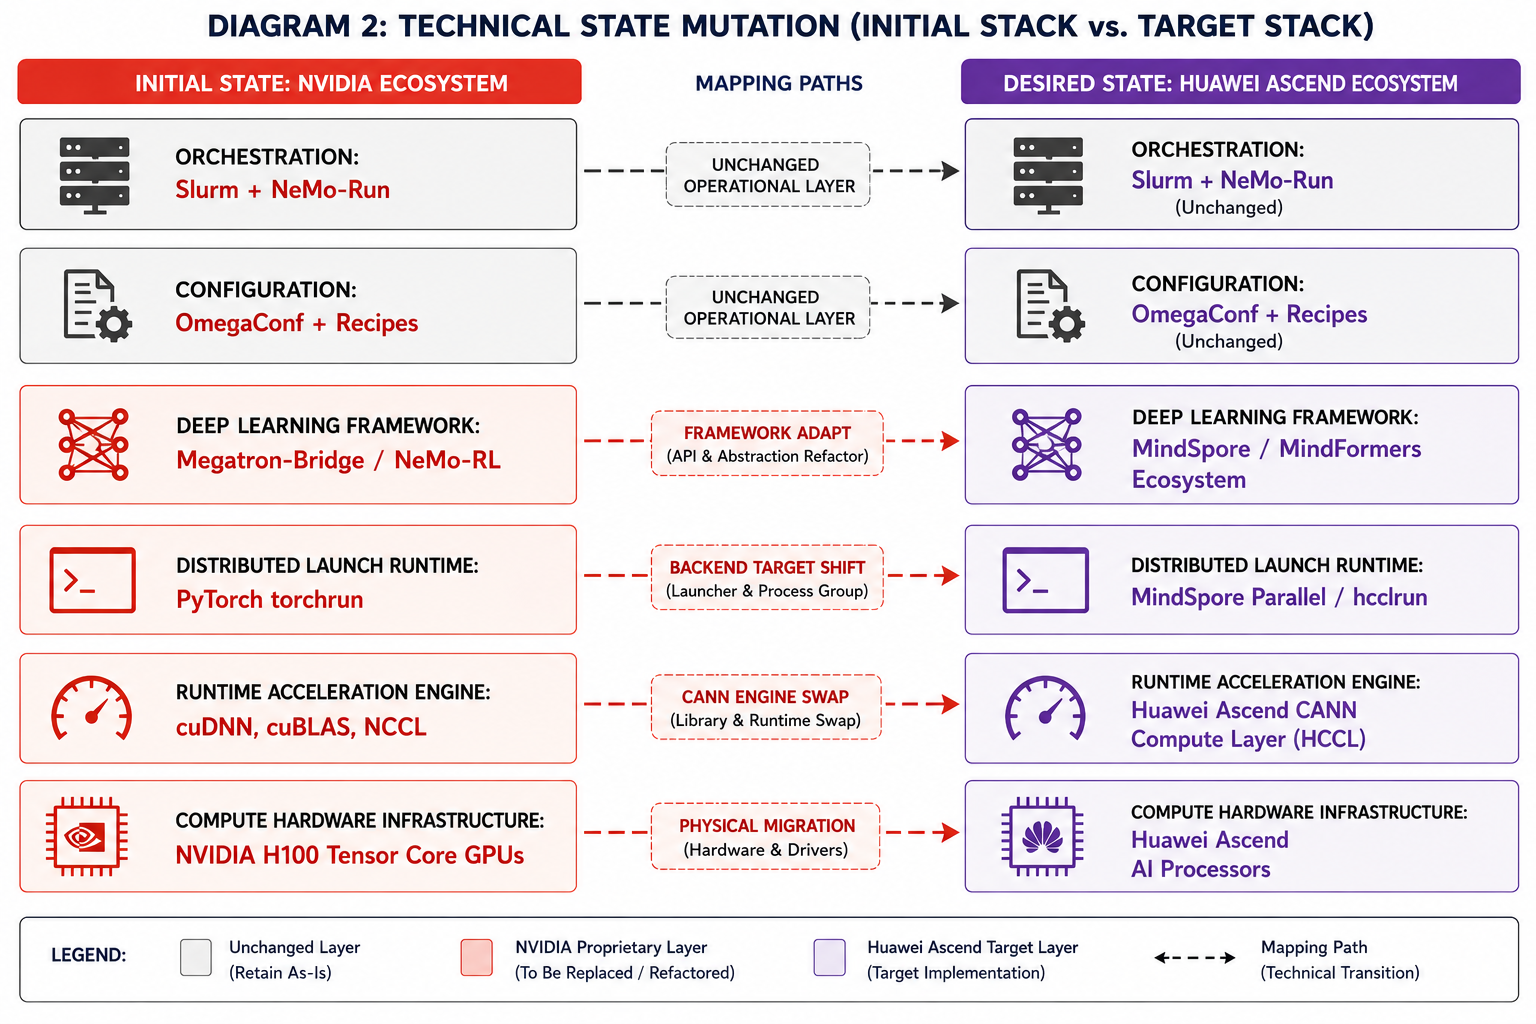
\includegraphics[width=0.85\textwidth]{images/figures/stack-mapping.png}
    \caption{CUDA-to-CANN Stack Mapping }
    \label{fig:CUDA-to-CANN Stack Mapping}
\end{figure}


\subsection{Two-Track Migration Strategy}
\label{subsec:two-tracks}

The migration follows a \term{two-track parallel-path strategy} that
separates correctness validation from production optimisation.

\textbf{Track A — PyTorch-NPU (validation track).} The
\texttt{torch\_npu} package registers Ascend as a PyTorch device
type (\texttt{"npu"}) and provides the \texttt{transfer\_to\_npu()}
monkey-patch that intercepts all \texttt{.cuda()} calls across the
entire Python process, including deep inside Megatron-Bridge. This
allows Megatron-Bridge to run on Ascend with minimal code changes.
The Mamba SSM and MoE operators are replaced with pure-PyTorch
fallback implementations that are correct on any device but
3--8$\times$ slower than the fused CUDA originals. Track A's
goal is to establish numerical correctness — a loss curve that
matches the CUDA baseline within 2\% — before any performance
optimisation.

\textbf{Track B — MindSpore-native (production track).} Full
reimplementation of model definition and training loops in
MindSpore with MindFormers, achieving maximum performance through
CANN-native graph execution with automatic operator fusion. Track B
is the production path but requires significantly more engineering
effort. It is developed in parallel with Track A, using Track A's
loss curves as the numerical correctness reference.

This project implements \textbf{Track A in full} — the complete,
runnable fine-tuning and inference pipeline — which constitutes
the primary deliverable. Track B is identified as future work,
with the correctness baseline established by Track A serving as its
acceptance reference.

\begin{figure}[H]
    \centering
    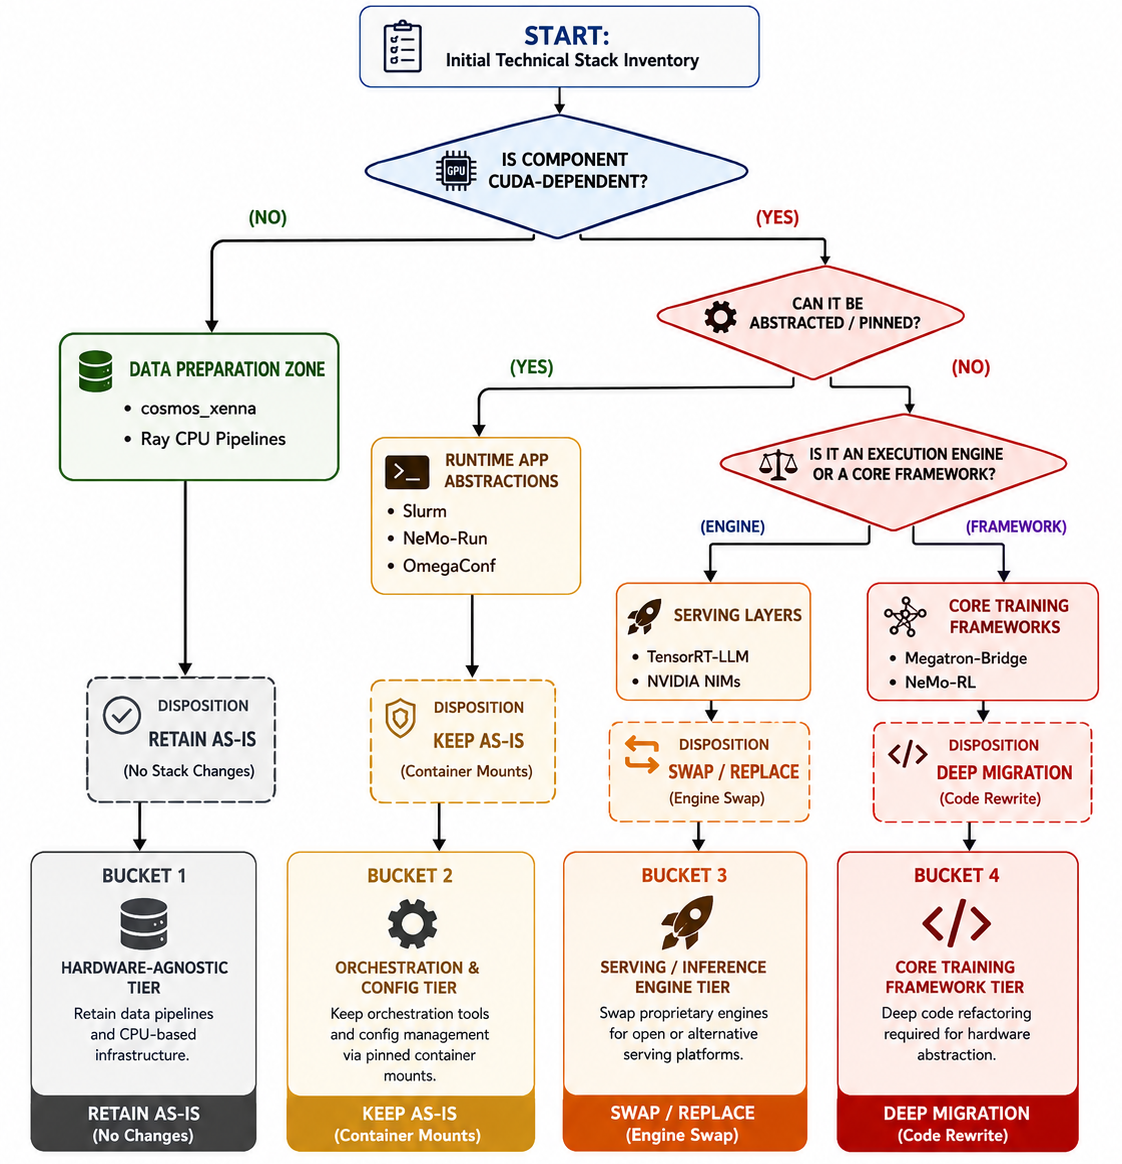
\includegraphics[width=0.85\textwidth]{images/figures/migration-strategy.png}
    \caption{Migration Strategy Overview}
    \label{fig:Migration Strategy Overview}
\end{figure}


\subsection{Cluster Configuration}
\label{sec:cluster-config}

All training and inference jobs are orchestrated via NeMo-Run and
Slurm. The \texttt{env.toml} file defines three execution profiles:
a single-node Ascend cluster (8 NPUs), a two-node Ascend cluster
(16 NPUs), and a baseline CUDA cluster. The Ascend profiles specify the
Slurm partition name, NPU device count, and required HCCL environment
variables (such as \texttt{HCCL\_BUFFSIZE} and \texttt{HCCL\_IF\_BASE\_PORT})
to ensure efficient collective communication.

\subsection{Container Strategy}
\label{sec:container-strategy}

Two custom Docker images are defined, replacing the NVIDIA NeMo
containers used in the original pipeline.

\textbf{\path{docker/Dockerfile.sft}} builds from
\path{ascendhub.huawei.com/public-ascendhub/ascend-pytorch},
installs \texttt{torch\_npu==2.1.0.post3} (pinned to match the
base image's PyTorch 2.1.0), clones and installs Megatron-Bridge
at a pinned commit, and copies the project source. The pinned
Megatron-Bridge commit (\texttt{bbbedbb9}) is the same commit
used in the original SFT stage, ensuring that framework-level
behaviour is identical between the CUDA and Ascend training runs.

\textbf{\path{docker/Dockerfile.inference}} builds from
\path{ascendhub.huawei.com/public-ascendhub/mindie:latest},
installs the FastAPI inference server dependencies (\texttt{uvicorn},
\texttt{pydantic}, \texttt{fastapi}), and copies \texttt{inference/}
and \texttt{tools/}. The \texttt{MODEL\_PATH}, \texttt{BACKEND},
and \texttt{DEVICES} parameters are injected at runtime via
environment variables, making the same image usable for both
MindIE and vLLM-Ascend backends without rebuilding.
